\begin{frame}{Byte-Pair Encoding (BPE)}
  \begin{itemize}
    \item[\textcolor{red}{$\blacktriangleright$}] \textbf{How BPE works:}
    \begin{itemize}
      \item Start with characters.
      \item Merge most frequent pair (e.g., ``t", ``h" $\rightarrow$ ``th").
      \item Repeat until vocab size reached.
    \end{itemize}
    \vspace{1em}
    \item[\textcolor{red}{$\blacktriangleright$}] \textbf{Advantages:}
    \begin{itemize}
      \item Handles unknown words well (e.g., unbelievably $\rightarrow$ un + believ + ably)
      \item Reduces sequence length
    \end{itemize}
    \vspace{1em}
    \item[\textcolor{red}{$\blacktriangleright$}] \textbf{Limitations:}
    \begin{itemize}
      \item Not optimal for all scripts (e.g., Chinese)
      \item Word boundaries may be unclear
    \end{itemize}
  \end{itemize}
\end{frame}

\begin{frame}{Byte-Pair Encoding (BPE)}
  \centering
  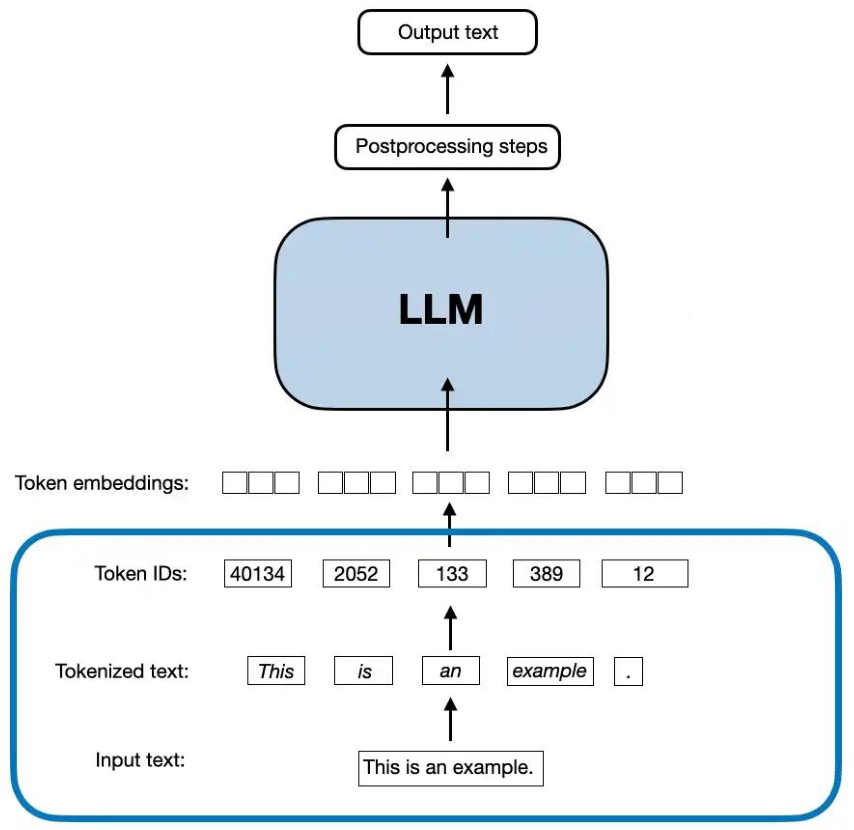
\includegraphics[width=0.60\paperwidth,height=0.60\paperheight,keepaspectratio]{images/large-language-models/llm_llm_tokenization_pipeline.png}
\end{frame}
